\chapter{Teakwood System }

\section{Overview}
\section{Frontend}
\section{Backend}
\section{Data handling}
\section{Remote Configuration}

%\subsection{<Sub-section title>}
%
%\subsection{<Sub-section title>}
%some text\cite{citation-2-name-here}, some more text
%\subsection{<Sub-section title>}
%
%\subsection{<Sub-section title>}

Refer figure \ref{fig:label}.

\begin{figure}[htb]
\centering
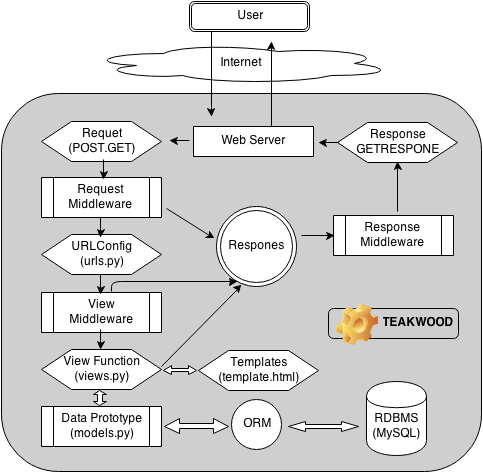
\includegraphics[scale=0.8]{./http_request_response}
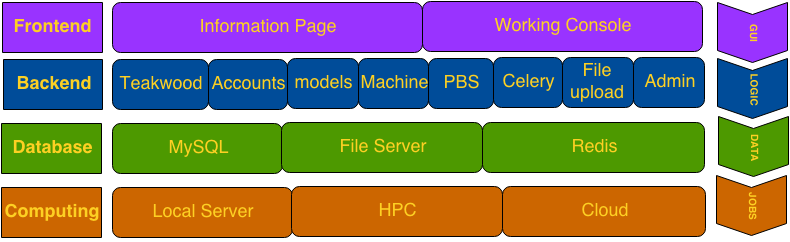
\includegraphics[scale=0.5]{./system_structure} 
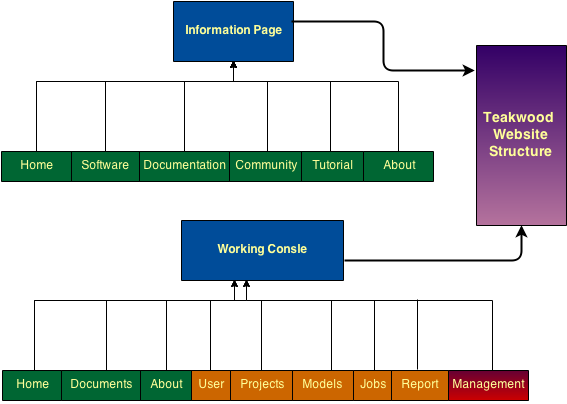
\includegraphics[scale=0.7]{./website_structure} % e.g. insert ./image for image.png in the working directory, adjust scale as necessary
\caption{<Caption here>}
\label{fig:label} % insert suitable label, this is used to refer to a fig from within the text as shown above
\end{figure}

